% Lily's Worship Songlist
\documentclass[10pt,oneside,footinclude=true,headinclude=true]{scrbook} % KOMA-Script book
\usepackage[LHE,T1]{fontenc}
\usepackage[linedheaders,nochapters]{classicthesis} % ,manychapters
\usepackage[paperheight=8.5in,paperwidth=5.5in,margin=0.8in]{geometry}
\usepackage{graphicx}

\usepackage[english]{babel}

\usepackage{paracol}
\usepackage{transparent}
\usepackage{cancel}
\usepackage{tikz}
\usetikzlibrary{calc}

% Helper functions.
\makeatletter
\newcommand{\verbatimfont}[1]{\renewcommand{\verbatim@font}{\rmfamily\normalsize}}
\makeatother

\newcommand\songtitle[1]{
	\hspace*{-3.7mm}\Large\textsc{#1}
}

\newcommand\pagequot[1]{
	\newpage
	\clearscrheadfoot
	%\vspace*{\fill}
	\vspace*{\stretch{2}}
	\begin{center}
	\begin{minipage}[c]{8cm}
		#1
	\end{minipage}
	\end{center}
	%\vspace*{\fill}
	\vspace*{\stretch{3}}
}


\begin{document}

\verbatimfont

%---------------------------------------------------------------------------------------
%	TITLE PAGE
%---------------------------------------------------------------------------------------
\begin{titlepage}
\begin{center}
\large \hfill \vfill

\begingroup
\color{RoyalPurple}\spacedallcaps{Lily's} \\
\bigskip
\color{RoyalPurple}\spacedallcaps{\huge{Worship Songlist}} \\ %Title
\bigskip
\endgroup

\bigskip\bigskip
\bigskip\bigskip
\bigskip\bigskip
\bigskip
%\spacedlowsmallcaps{Lily Jusman}
%\vfill
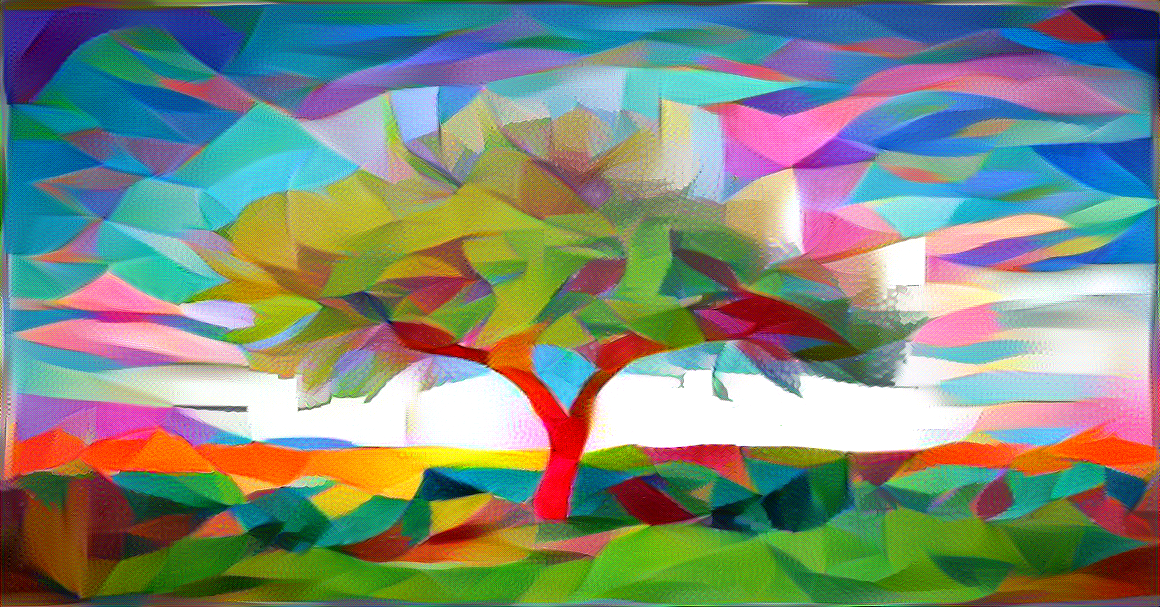
\includegraphics[width=10cm]{GSITree-triangle.png} \\
%\vfill
\bigskip
\bigskip\bigskip
\bigskip\bigskip
\bigskip\bigskip

\textit{...The leaves of the tree were for the healing of the nations....} \\ \medskip % Subtitle

October 2018\ -- version 1.0 % Time and version

\vfill
\end{center}
\end{titlepage}
    
%\newpage
%\clearscrheadfoot
%\null


%---------------------------------------------------------------------------------------
%	TOC
%---------------------------------------------------------------------------------------
%\tableofcontents 
%\cleardoublepage % use \cleardoublepage here to avoid problems with pdfbookmark


%---------------------------------------------------------------------------------------
%	SONGS
%---------------------------------------------------------------------------------------

%---------------------------------------------------------------------------------------

\songtitle{Amazing Grace}
\begin{verbatim}
by John Newton

Amazing grace! How sweet the sound
That saved a wretch like me!
I once was lost, but now am found;
Was blind, but now I see.

'Twas grace that taught my heart to fear,
And grace my fears relieved;
How precious did that grace appear
The hour I first believed.

Through many dangers, toils and snares,
I have already come;
'Tis grace hath brought me safe thus far,
And grace will lead me home.

The Lord has promised good to me,
His Word my hope secures;
He will my Shield and Portion be,
As long as life endures.

Yea, when this flesh and heart shall fail,
And mortal life shall cease,
I shall possess, within the veil,
A life of joy and peace.

The earth shall soon dissolve like snow,
The sun forbear to shine;
But God, who called me here below,
Will be forever mine.

When we've been there ten thousand years,
Bright shining as the sun,
We've no less days to sing God's praise
Than when we'd first begun.
\end{verbatim}

%---------------------------------------------------------------------------------------

\bigskip
\songtitle{Be Thou My Vision}
\begin{verbatim}
by Dallan Forgaill

Be Thou my Vision, O Lord of my heart;
Naught be all else to me, save that Thou art;
Thou my best Thought, by day or by night,
Waking or sleeping, Thy presence my light.

Be Thou my Wisdom, and Thou my true Word;
I ever with Thee and Thou with me, Lord;
Thou my great Father, I Thy true son;
Thou in me dwelling, and I with Thee one.

Be Thou my battle Shield, Sword for the fight;
Be Thou my Dignity, Thou my Delight;
Thou my soul's Shelter, Thou my high Tow'r:
Raise Thou me heav'nward, O Pow'r of my pow'r.

Riches I heed not, nor man's empty praise,
Thou mine Inheritance, now and always:
Thou and Thou only, first in my heart,
High King of Heaven, my Treasure Thou art.

High King of Heaven, my victory won,
May I reach Heaven's joys, O bright Heav'n's Sun!
Heart of my own heart, whatever befall,
Still be my Vision, O Ruler of all.
\end{verbatim}

%---------------------------------------------------------------------------------------

\bigskip
\medskip
\songtitle{Because He Lives}
\begin{verbatim}
by Gloria & William Gaither

God sent His son, they called Him Jesus
He came to love, heal and forgive
He lived and died to buy my pardon
An empty grave is there to prove my savior lives

Because He lives, I can face tomorrow
Because He lives, all fear is gone
Because I know He holds the future
And life is worth the living, just because He lives

How sweet to hold a newborn baby
And feel the pride and joy He gives
But greater still the calm assurance
This child can face uncertain day, because He lives

Because He lives...

And then one day, I'll cross the river
I'll fight life's final war with pain
And then, as death gives way to victory
I'll see the lights of glory and I'll know He reigns

Because He lives... (2x)
\end{verbatim}

%---------------------------------------------------------------------------------------

\bigskip
\medskip
\songtitle{Blessed Be Your Name}
\begin{verbatim}
by Beth & Matt Redman

Blessed Be Your Name
In the land that is plentiful
Where Your streams of abundance flow
Blessed be Your name

Blessed Be Your name
When I'm found in the desert place
Though I walk through the wilderness
Blessed Be Your name

Every blessing You pour out, I'll
Turn back to praise
When the darkness closes in, Lord
Still I will say

Blessed be the name of the Lord
Blessed be Your name
Blessed be the name of the Lord
Blessed be Your glorious name

Blessed be Your name
When the sun's shining down on me
When the world's 'all as it should be'
Blessed be Your name

Blessed be Your name
On the road marked with suffering
Though there's pain in the offering
Blessed be Your name

Every blessing You pour out I'll...

Blessed be the name of the Lord... (2x)

You give and take away
You give and take away
My heart will choose to say
Lord, blessed be Your name

You give and take away...

Blessed be the name of the Lord... (2x)
\end{verbatim}

%---------------------------------------------------------------------------------------

\bigskip
\medskip
\songtitle{Breathe}
\begin{verbatim}
by Liam Howe, Thaliah Barnett, & Timmaz Zolleyn

This is the air I breathe
This is the air I breathe
Your holy presence living in me

This is my daily bread
This is my daily bread
Your very word spoken to me

And I... I'm desperate for you
And I... I'm lost without you

(Repeat from beginning)

I'm lost without you...
I'm desperate for you...
\end{verbatim}

%---------------------------------------------------------------------------------------

\bigskip
\medskip
\songtitle{Cornerstone}
\begin{verbatim}
by Eric Liljero, Jonas Myrin, & Reuben Morgan

My hope is built on nothing less
Than Jesus' blood and righteousness
I dare not trust the sweetest frame
But wholly trust is Jesus' name

My hope is built on nothing less
Than Jesus' blood and righteousness
I dare not trust the sweetest frame
But wholly trust is Jesus' name

Christ alone, Cornerstone
Weak made strong in the Savior's love
Through the storm, He is Lord
Lord of all

When darkness seems to hide His face
I rest on His unchanging grace
In every high and stormy gale
My anchor holds within the veil
My anchor holds within the veil

Christ alone, Cornerstone... (3x)

When he shall come with trumpet sound
Oh, may I then in Him be found
Dressed in His righteousness alone
Faultless, stand before the throne

Christ alone, Cornerstone... (2x)
\end{verbatim}

%---------------------------------------------------------------------------------------

\bigskip
\medskip
\songtitle{El Shaddai}
\begin{verbatim}
by Michael Card & John Thompson

El shaddai, el shaddai,
El-elyon na adonia,
Age to age you're still the same,
By the power of the name.

El shaddai, el shaddai,
Erkamka na adonai,
We will praise and lift you high,
El shaddai.

Through your love and through the ram,
You saved the son of abraham;
Through the power of your hand,
Turned the sea into dry land.

To the outcast on her knees,
You were the God who really sees,
And by your might,
You set your children free.

El shaddai, el shaddai...

Through the years you've made it clear,
That the time of christ was near,
Though the people couldn't see
What messiah ought to be.

Though your word contained the plan,
They just could not understand
Your most awesome work was done
Through the frailty of your son.

El shaddai, el shaddai... (3x)
\end{verbatim}

%---------------------------------------------------------------------------------------

\bigskip
\medskip
\songtitle{Here I Am To Worship}
\begin{verbatim}
by Mark Hayes & Tim Hughes

Light of the world, You stepped down into darkness
Opened my eyes, let me see
Beauty that made this heart adore You
Hope of a life spent with You

Here I am to worship, Here I am to bow down
Here I am to say that You're my God
You're altogether lovely, Altogether worthy
Altogether wonderful to me

King of all days, Oh so highly exalted
Glorious in heaven above
Humbly You came to the earth You created
All for love's sake became poor

Here I am to worship...

Well, I'll never know how much it cost
To see my sin upon that cross
(Repeat 3x)
\end{verbatim}

%---------------------------------------------------------------------------------------

\bigskip
\medskip
\songtitle{How Great Thou Art}
\begin{verbatim}
by Carl Boberg

O Lord my God, When I in awesome wonder
Consider all The works Thy Hand hath made,
I see the stars, I hear the mighty thunder,
Thy pow'r throughout The universe displayed,

When through the woods And forest glades I wander
I hear the birds Sing sweetly in the trees,
When I look down From lofty mountain grandeur
And hear the brook And feel the gentle breeze,

Then sings my soul, My Savior God, to Thee,
How great Thou art! How great Thou art!
Then sings my soul, My Savior God, to Thee,
How great Thou art! How great Thou art!

When Christ shall come, With shouts of acclamation,
And take me home, What joy shall fill my heart!
Then I shall bow In humble adoration
And there proclaim, "My God, how great Thou art!"

Then sings my soul...
\end{verbatim}

%---------------------------------------------------------------------------------------

\bigskip
\medskip
\songtitle{I Surrender All}
\begin{verbatim}
by Winfield Weeden & Judson Van Deventer

All to Jesus I surrender
All to Him I freely give
I will ever love and trust Him
In His presence daily live

All to Jesus I surrender
Humbly at His feet I bow
Worldly pleasures all forsaken
Take me, Jesus, take me now,

I surrender all
I surrender all
All to Thee my blessed Savior
I surrender all

All to Jesus I surrender
Make me Savior wholly thine
May Thy Holy Spirit fill me
May I know Thy power divine

I surrender all... (2x)
\end{verbatim}

%---------------------------------------------------------------------------------------

\bigskip
\medskip
\songtitle{In Christ Alone}
\begin{verbatim}
by Keith Getty & Stuart Townend

In Christ alone my hope is found
He is my light, my strength, my song
This cornerstone, this solid ground,
Firm through the fiercest drought and storm.

What heights of love, what depths of peace,
When fears are stilled, when strivings cease!
My comforter, my all in all
Here in the love of Christ I stand.

In Christ alone, Who took on flesh,
Fullness of God in helpless babe!
This gift of love and righteousness,
Scorned by the ones He came to save.

'Til on that cross as Jesus died,
The wrath of God was satisfied
For ev'ry sin on Him was laid
Here in the death of Christ I live.

There in the ground His body lay,
Light of the world by darkness slain
Then bursting forth in glorious day,
Up from the grave He rose again!

And as He stands in victory,
Sin's curse has lost its grip on me
For I am His and He is mine
Bought with the precious blood of Christ.

No guilt in life, no fear in death
This is the pow'r of Christ in me
From life's first cry to final breath,
Jesus commands my destiny.

No pow'r of hell, no scheme of man,
Can ever pluck me from His hand
'Til He returns or calls me home
Here in the pow'r of Christ I'll stand.
\end{verbatim}

%---------------------------------------------------------------------------------------

\bigskip
\medskip
\songtitle{Is He Worthy}
\begin{verbatim}
by Andrew Peterson & Ben Shive

Do you feel the world is broken?  (We do)
Do you feel the shadows deepen?  (We do)
But do you know that all the dark won't stop
  the light from getting through?  (We do)
Do you wish that you could see it all made new?  (We do)

Is all creation groaning?  (It is)
Is a new creation coming?  (It is)
Is the glory of the Lord to be the light within our midst?  (It is)
Is it good that we remind ourselves of this?  (It is)

Is anyone worthy? Is anyone whole?
Is anyone able to break the seal and open the scroll?
The Lion of Judah who conquered the grave
He is David's root and the Lamb who died to ransom the slave

Is He worthy? Is He worthy?
Of all blessing and honor and glory
Is He worthy of this?
He is

Does the Father truly love us?  (He does)
Does the Spirit move among us?  (He does)
And does Jesus, our Messiah hold forever those He loves?  (He does)
Does our God intend to dwell again with us?  (He does)

Is anyone worthy? Is anyone whole?...

From every people and tribe
Every nation and tongue
He has made us a kingdom and priests to God
To reign with the Son

Is He worthy? Is He worthy?...

Is He worthy? Is He worthy?
He is!
He is!
\end{verbatim}

%---------------------------------------------------------------------------------------

\bigskip
\medskip
\songtitle{It Is Well With My Soul}
\begin{verbatim}
by Horatio G Spafford

When peace, like a river, attendeth my way,
When sorrows like sea billows roll;
Whatever my lot, Thou hast taught me to say,
It is well, it is well with my soul.

It is well with my soul,
It is well, it is well with my soul.

Though Satan should buffet, though trials should come,
Let this blest assurance control,
That Christ hath regarded my helpless estate,
And hath shed His own blood for my soul.

It is well with my soul...

My sin --oh, the bliss of this glorious thought!--
My sin, not in part but the whole,
Is nailed to the cross, and I bear it no more,
Praise the Lord, praise the Lord, O my soul!

It is well with my soul...

For me, be it Christ, be it Christ hence to live:
If Jordan above me shall roll,
No pang shall be mine, for in death as in life
Thou wilt whisper Thy peace to my soul.

It is well with my soul...

But, Lord, 'tis for Thee, for Thy coming we wait,
The sky, not the grave, is our goal;
Oh, trump of the angel! Oh, voice of the Lord!
Blessed hope, blessed rest of my soul!

It is well with my soul...

And Lord, haste the day when the faith shall be sight,
The clouds be rolled back as a scroll;
The trump shall resound, and the Lord shall descend,
Even so, it is well with my soul.

It is well with my soul...
\end{verbatim}

%---------------------------------------------------------------------------------------

\bigskip
\medskip
\songtitle{Knowing You}
\begin{verbatim}
by Graham Kendrick

All I once held dear, built my life upon
All this world reveres, and wars to own
All I once thought gain, I have counted loss
Spent and worthless now, compared to this

Knowing you, Jesus, knowing you
There is no greater thing
You're my all, you're the best
You're my joy, my righteousness
And I love you, Lord

Now my heart's desire is to know you more
To be found in you and known as yours
To possess by faith what I could not earn
All-surpassing gift of righteousness

Knowing you, Jesus, knowing you...

Oh, to know the power of your risen life
And to know You in Your sufferings
To become like you in your death, my Lord
So with you to live and never die

Knowing you, Jesus, knowing you...
\end{verbatim}

%---------------------------------------------------------------------------------------

\bigskip
\medskip
\songtitle{Lord I Need You}
\begin{verbatim}
by Matt Maher

Lord, I come, I confess
Bowing here I find my rest
Without You I fall apart
You're the One that guides my heart

Lord, I need You, oh, I need You
Every hour I need You
My one defense, my righteousness
Oh God, how I need You

Where sin runs deep Your grace is more
Where grace is found is where You are
Where You are, Lord, I am free
Holiness is Christ in me

Lord, I need You, oh, I need You...

So teach my song to rise to You
When temptation comes my way
When I cannot stand I'll fall on You
Jesus, You're my hope and stay

Lord, I need You, oh, I need You... (2x)
\end{verbatim}

%---------------------------------------------------------------------------------------

\newpage
\songtitle{Power Of Your Love}
\begin{verbatim}
by Geoff Bullock

Lord I come to You
Let my heart be changed, renewed
Flowing from the grace
That I've found in You

Lord I've come to know
The weaknesses I see in me
Will be stripped away
By the power of Your love

Hold me close
Let Your love surround me
Bring me near
Draw me to Your side
And as I wait
I'll rise up like the eagle
And I will soar with You
Your Spirit leads me on
In the power of Your love

Lord unveil my eyes
Let me see You face to face
The knowledge of Your love
As You live in me

Lord renew my mind
As Your will unfolds in my life
In living every day
By the power of Your love

Hold me close... (2x)
\end{verbatim}

%---------------------------------------------------------------------------------------

\newpage
\songtitle{The Old Rugged Cross}
\begin{verbatim}
by George Bennard

On a hill far away stood an old rugged cross,
The emblem of suff'ring and shame;
And I love that old cross where the Dearest and Best
For a world of lost sinners was slain.

So I'll cherish the old rugged cross,
Till my trophies at last I lay down;
I will cling to the old rugged cross,
And exchange it someday for a crown.

Oh, that old rugged cross, so despised by the world,
Has a wondrous attraction for me;
For the dear Lamb of God left His glory above
To bear it to dark Calvary.

So I'll cherish the old rugged cross...

In that old rugged cross, stained with blood so divine,
A wondrous beauty I see,
For 'twas on that old cross Jesus suffered and died,
To pardon and sanctify me.

So I'll cherish the old rugged cross...

To the old rugged cross I will ever be true;
Its shame and reproach gladly bear;
Then He'll call me someday to my home far away,
Where His glory forever I'll share.

So I'll cherish the old rugged cross...
\end{verbatim}

%---------------------------------------------------------------------------------------

\newpage
\songtitle{Tis So Sweet}
\begin{verbatim}
by William James Kirkpatrick, Canzetta Staton, & Louisa M. Stead

'Tis so sweet to trust in Jesus,
Just to take Him at His Word
Just to rest upon His promise,
Just to know, "Thus saith the Lord!"

Jesus, Jesus, how I trust Him!
How I've proved Him o'er and o'er
Jesus, Jesus, precious Jesus!
Oh, for grace to trust Him more!

I'm so glad I learned to trust Him,
Precious Jesus, Savior, Friend
And I know that He is with me,
Will be with me to the end.

Oh, how sweet to trust in Jesus,
Just to trust His cleansing blood
And in simple faith to plunge me
'Neath the healing, cleansing flood!

Yes, 'tis sweet to trust in Jesus,
Just from sin and self to cease
Just from Jesus simply taking
Life and rest, and joy and peace.
\end{verbatim}

%---------------------------------------------------------------------------------------

\bigskip
\medskip
\songtitle{You Are My All In All}
\begin{verbatim}
by Dennis Jernigan

You are my strength when I am weak
You are the treasure that I seek
You are my all in all
Seeking You as a precious jewel
Lord to give up I'd be a fool
You are my all in all

Jesus Lamb of God worthy is your name (2x)

Taking my sin my cross my shame
Rising again I bless your name
You are my all in all
When I fall down you pick me up
When I am dry You fill my cup
You are my all in all

Jesus Lamb of God worthy is your name (4x)
\end{verbatim}

%---------------------------------------------------------------------------------------

\bigskip
\medskip
\songtitle{You Raise Me Up}
\begin{verbatim}
by Brendan Graham & Rolf Lovland

When I am down and, oh my soul, so weary
When troubles come and my heart burdened be
Then, I am still and wait here in the silence
Until you come and sit awhile with me

You raise me up, so I can stand on mountains
You raise me up, to walk on stormy seas
I am strong, when I am on your shoulders
You raise me up... To more than I can be

You raise me up, so I can stand on mountains...

There is no life - no life without its hunger
Each restless heart beats so imperfectly
But when you come and I am filled with wonder
Sometimes, I think I glimpse eternity

You raise me up, so I can stand on mountains... (2x)
You raise me up, to walk on stormy seas
I am strong, when I am on your shoulders
You raise me up... To more than I can be
\end{verbatim}

%---------------------------------------------------------------------------------------

\end{document}
